%% LaTeX2e class for student theses
%% sections/content.tex
%% 
%% Karlsruhe Institute of Technology
%% Institute for Program Structures and Data Organization
%% Chair for Software Design and Quality (SDQ)
%%
%% Dr.-Ing. Erik Burger
%% burger@kit.edu
%%
%% Version 1.2, 2016-09-20


\chapter{Device Manufacturing: Local Deposition}
\label{ch:ew}
Organic materials are processed in a different manner than inorganic materials. While inorganic materials have to be processed, for the most part, by means such as physical vapor deposition, cathodic arc deposition or electrospray deposition, to name a few, organic materials have the advantage of being not only deposed but also printed. In the present work, an automated method for local material deposition is implemented. 

\section{Current State}

Local deposition means that a polymer dissolved in a liquid is passed through a slit or a slot, which is filled with the electro-optical chromophore, and then developed for further processing.

For the local deposition of materials, a set of stepper motors with fine steps are utilized and driven with a \textbf{ESP300 Motion Controller/Driver} manufactured by Newport, which allows for 3-axis movement and positioning of devices. A general chip layout is shown in figure \ref{fig:chiplo}. A right-hand cartesian coordinate system is chosen, such that the chip is visualized with a camera, and the movement corresponds to the spatial shift observed through the camera (i.e. if the motor system is "reversed" then movements are mirrored in software).  \par\medskip

The most important offsets and distances indicated in figure \ref{fig:chiplo} are the following:
\begin{itemize}
	\item $\mathbf{d_n}$, which is the length of a specific device that needs to be processed. This has been set as a variable since a single chip may contain different device lengths, but is not common to have different lengths along the $y$-axis.
	\item  $\mathbf{d_n/2}$ is the middle point of a device, and this is the region where the droplet is prepared as it is far from the optical devices but has a relatively equal surface height to avoid changes in the droplet size.
	\begin{itemize}
		\item In some cases, a position $\mathbf{x^*_n}$ can be used in case a specific overlap with a sensitive optical device occurs at the middle of the device. Further, this will be the offset of choice to describe the positioning as it is the most generalized position. 
	\end{itemize}
	\item $\mathbf{y_q}$ is the distance in the $y$-axis in which the droplet is prepared for deposition, and $\mathbf{y_p}$ is the device pitch (i.e. distance between two devices).   
\end{itemize}

\begin{figure}[!ht]
\centering
  \includestandalone[width=0.8\textwidth]{tikz/chiplo}
  \caption{Chip layout for local deposition. (0,0) indicates the chip origin.}
  \label{fig:chiplo}
\end{figure}

Figure \ref{fig:zaxislo} shows the layout of the vertical axis, in which the chip surface, at position $z_0$, is going to be subject to local deposition using a biomedical grade needle. The needle is previously wetted with the polymer solution of interest and the chip is allocated in the chip mount. By using a camera, the height $z_v$ is the height at which the needle is visible through the camera. The needle is positioned at $(x^*_n, q_n,z_v)$. The needle is approximated to the surface $z_0$ using steps $\Delta z$ in order to avoid direct contact with the optical layout (as the needle can easily bend and break, or damage the optical devices). The position can be detected by direct visualization. Once the needle is at exactly $z_0$, the needle is slowly lifted to $z_m$ to form the meniscus\footnote{in the figure, the shape utilized to picture the meniscus is a gaussian, as this proved to be the the fastest solution to show the meniscus on both sides exploiting the layering capabilities of TiKz. This, however, is not an accurate representation of the physical phenomenon due to surface tension which has a form closer to a cosine. For schematic purposes, though, the meniscus is adequately represented by the gaussian used in the figure.} which will depose the polymer into the slot. The needle is then moved along the $x$-axis along the device to deposit the material into the slot twice, and the needle is lifted to position $z_v$. The organic polymer should be deposited only in the slot since it can produce undesired effects after the electrical packaging.

%A semi-automatic mode is implemented to approach the needle to the surface. There is no collision warning or lock-out conditions for the basic implementation. 

\begin{figure}[!ht]
\centering
  \includestandalone[width=0.7\textwidth]{tikz/zaxislo}
  \caption{$z$-axis layout for local deposition.}
  \label{fig:zaxislo}
\end{figure}

\section{Local Deposition Method}

%\subsection{Process Flow}

%The main process flow is detailed in figure \ref{fig:ldbd}. 

%\begin{figure}[!ht]
%\centering
%  \includestandalone[width=0.7\textwidth]{tikz/ldbd}
%  \caption{Local deposition block diagram.}
%  \label{fig:ldbd}
%\end{figure}

%\subsection{Software Requirements}

%\clearpage
%\newpage
%% Schematic representation of mach zender interferometer
% Modified from a version created by Henrik Kröger, https://github.com/derhedwig/fiberoptics/blob/master/auswertung.tex
% Author: Orlando Torres (2016)

\documentclass[12pt,a4paper,preview]{standalone}
\usepackage{amsmath} % Required for \varPsi below
\usepackage{tikz,pgfplots}
\usetikzlibrary{calc}
\usetikzlibrary{patterns}
\usetikzlibrary{backgrounds}
\usepackage{caption}
\usepackage{booktabs}
\usepackage{multirow}
\usepackage{siunitx}
\usepackage{rotating}
\usepackage{pdflscape}
\usepackage{array} 
\usepackage{graphicx}
%\sisetup{binary-units = true,table-format=7.0}

\begin{document}

\begin{landscape}
%\minipage{1.08\textwidth}
%\addtolength{\tabcolsep}{-1.0pt}
\begin{table}[htbp]
\centering
\newcommand*{\tpb}[1]{{\parbox[c]{10cm}{\raggedright #1}}}%
\newcommand*{\tpd}[1]{{\parbox[c]{4cm}{\raggedright #1}}}%
\scalebox{0.9}{
\begin{tabular}{@{}lllll@{}}
\toprule
ID & Feature                          & Description                                                                                                                                                                      & Priority & Status \\ \midrule
1  & \tpd{Automatic Dispensing }            & \tpb{The dispense mechanism for polymers is mostly automated. }                                                                                                                        & Top      & Open   \\\midrule
2  & \tpd{Double Slot Deposition }          & \tpb{Dispense mechanism can deposit a polymer on a double slot simultaneously  }                                                                                                       & High     & Open   \\\midrule
3  & \tpd{Column Deposition }               & \tpb{Dispense mechanism can deposit a polymer on a double slot simultaneously in an column of equally-sized devices        }                                                           & High     & Open   \\\midrule
4  & \tpd{Multi-column Deposition }         & \tpb{Dispense mechanism can deposit a polymer on a double slot simultaneously in multiple columns of equally-sized devices  }                                                          & High     & Open   \\\midrule
5  & \tpd{$z$-axis tolerancing }            & \tpb{Take into account leveling differences of the chip due to manufacturing tolerances to avoid device damage or needle breakage.   }                                                 & Low      & Open   \\\midrule
6  & \tpd{$xy$-axis tolerancing}            & \tpb{Take into account $xy$-plane alignment of the device for roll, pitch and yaw (rotations in $x$-, $y$- and $z$-axis, respectively) }                                               & Medium   & Open   \\\midrule
7  & \tpd{Multiple Polymer Dispensing }     & \tpb{Enable the user to dispense multiple types of polymer at specific columns or row sets.}                                                                                           & Low      & Open   \\\midrule
8  & \tpd{Matrix Deposition}                & \tpb{Dispense mechanism can have different column, row, and device settings in the advanced menu.} 																			& Low      & Open   \\\midrule
9  & \tpd{Height Detection  }               & \tpb{Use PID controller feedback in the motor driver to detect collision.}                                                                                                             & Low      & Open   \\\midrule
10 & \tpd{Report Generation}                & \tpb{Generate report of activities with time stamps, total duration of deposition, location of polymers, device sizes, offsets, and general calculations and detections.}              & Medium   & Open   \\\midrule
11 & \tpd{Camera Visualization  }           & \tpb{Visualize the current layout using one of the cameras directly connected to the driving computer.  }                                                                              & Medium   & Open   \\\midrule
12 & \tpd{Full Field-of-View Visualization} & \tpb{Use a network arrangement to be able to observe both cameras at the same time using a single screen.   }                                                                          & Low      & Open   \\\midrule
13 & \tpd{Image Processing}                 & \tpb{Automated detection of offsets, locations, distances and devices.               }                                                                                                 & Low      & Open   \\ \bottomrule
\end{tabular}
}
\caption{Software requirements decision matrix.}
\label{table:softreqs}
\end{table}
\end{landscape}
%\end{sidewaystable}

\end{document}
%\clearpage
%\newpage

%\subsection{Security Requirements}

%The software developed should cover security features, implemented in order to avoid the damaging a chip. 

%The security requirements are detailed in the following list:

%\begin{itemize}
%\item \textbf{Collision warning:} Warns the user about a possible collision due to the following causes:
%	\begin{itemize}
%	\item The chip is moved towards the needle positioned to close to $z_0$ in the $xy$-plane (reference $z$-plane), meaning the needle could potentially move the chip from its position or break.
%	\item The chip is moved towards the needle positioned to close to $z_0$ in the $z$-plane (reference $z$-plane), meaning the needle could potentially bend and break due to excessive force applied and damage the chip.
%	\end{itemize}
%\item \textbf{Lock-out Condition:} This condition stops the machine at any condition that could potentially damage the chip without user interaction, such as reaching boundary positions or critical damage locations.
%%\end{itemize}

%\subsection{ESP300 Motion Controller/Driver}

%For the implementation of ESP300 functions, a few were not included due to the following reasons:

%\begin{itemize}
%\item \textbf{DIO Bit interactions:} Such as enabling or disabling motion, notifications, motion status, jog direction, etc. Are %not implemented because the direct control of GPIB is outside the scope of this experimental work and there is no specific request to have an external controller (other than the one provided in the motion controller itself) for this specific device.
%\item \textbf{Synchronized movement:} The ESP300 controller showed several problems when trying to move two axes (or three) at the same time. This reduces slightly the 
%\end{itemize}

\subsection{Graphic User Interface Improvements}

The local deposition software was refreshed to adress the following issues:

\begin{itemize}
\item Constant software shutdown
\item Improved control schemes
\item Faster positioning
\end{itemize}

\begin{figure}[!ht]
\centering
\begin{tabular}{cc}
\subfloat[Top GUI]{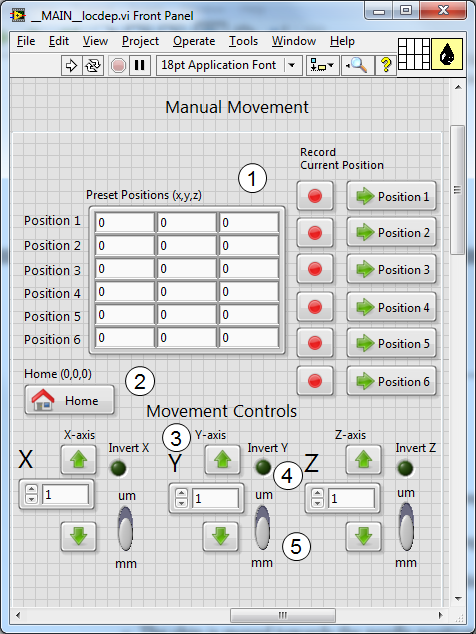
\includegraphics[width=0.4\textwidth]{figs/LOCDEP_top}\label{LDtop}} &
\subfloat[Bottom GUI]{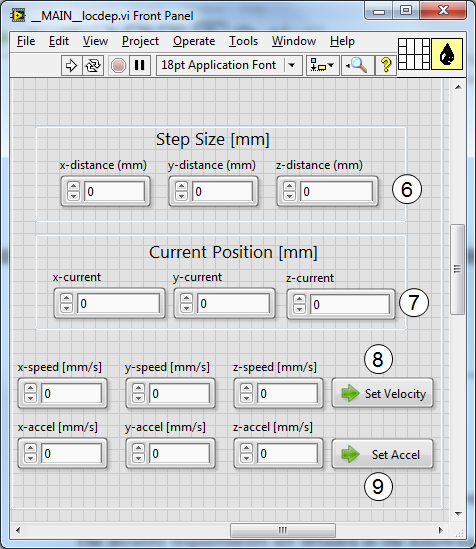
\includegraphics[width=0.4\textwidth]{figs/LOCDEP_bot}\label{LDbot}} \\
%\subfloat[]{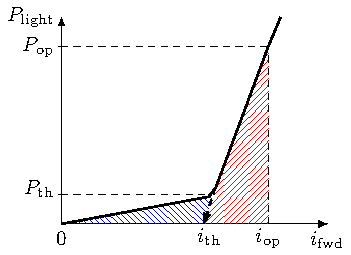
\includegraphics[width=0.4\textwidth]{tikz/LIcurve}} &
%\subfloat[]{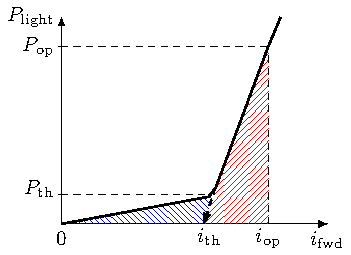
\includegraphics[width=0.4\textwidth]{tikz/LIcurve}} 
\end{tabular}
\caption{Local deposition GUI.}
\label{fig:locdep}
\end{figure}

The componenents of the GUI are the following:

\begin{enumerate}
\item \textbf{Preset positions}: Allows the user to record specific positions in the chip field which are commonly used to allow for faster navigation in the chip. The red button is used to record the current position, and the green arrow goes to the specific position. 
\item \textbf{Home}: Goes to the ``Home'' position at (0,0,0). The flow always starts by moving the $z$-axis before moving the $x$ and $y$ axes, for security purposes.
\item \textbf{Movement controls}: The arrows move in the positive direction with respect to the home position (0,0,0). This means that, when the button going up is pressed, the motors will move in the positive direction, the number of units in the number field between the two arrows. 
\item \textbf{Invert movement}: This button, when enabled (light is ``ON''), will move in the opposite direction. This was implemented since the $z$-axis considers moving in the positive direction as ``moving down'', which can be confusing for some users.
\item \textbf{Magnitude switch}: This changes the units of movement from millimeters to micrometers depending on the position of the rocker. 
\item \textbf{Step size}: Shows the step size calculated from the parameters in the movement controls.
\item \textbf{Current position}: Shows the step size calculated from the parameters input the movement controls.
\item \textbf{Set velocity}: Select the final velocity of each axis separately.
\item \textbf{Set velocity}: Select the acceleration of each axis separately.
\end{enumerate}